\chapter{Aufgabe 2}

\section{Teil 1}

\textit{Geben Sie die Schaltfunktionen von $y_3$, $y_2$ und $y_1$ an.}\\


\noindent

\noindent
Zur Erstellung der Schaltfunktionen für die jeweiligen Ausgänge $y_3$, $y_2$, $y_1$ überführen wir zeilenweise in die DNF.\\
Hierzu bilden wir für die jeweiligen Ausgänge die Minterme\footnote{
    ``für genau eine Variablenbelegung wahr``~\cite[92]{Hof22}
} und verknüpfen sie dann disjunktiv (Ziffern in Klammern beziehen sich auf die Zeilen der in der Aufgabenstellung angegebenen Tabelle).\\

\noindent
Für $y_3$ erhalten wir die DNF wie in~\ref{eq:dnf_y3} angegeben:


\begin{equation}\label{eq:dnf_y3}
\begin{alignat}{3}
    y_3 =\ &(\neg a \ \land \phantom{\neg} b \ \land \phantom{\neg} c \ \land \phantom{\neg} d)\ \lor && \text{(7)} \\
          &(\phantom{\neg} a \ \land \phantom{\neg} b \ \land \phantom{\neg} c \ \land \neg d) && \text{(14)}
\end{alignat}
\end{equation}

\noindent
Für $y_2$ erhalten wir die DNF wie in~\ref{eq:dnf_y2} angegeben:


\begin{equation}\label{eq:dnf_y2}
\begin{alignat}{3}
    y_2 =\ &(\neg a \ \land \phantom{\neg} b \ \land \neg c \ \land \phantom{\neg} d)\ \lor && \text{(5)} \\
    &(\phantom{\neg} a \ \land \neg b \ \land \neg c \ \land \phantom{\neg} d)\ \lor && \text{(9)}  \\
    &(\phantom{\neg} a \ \land \neg b \ \land  \phantom{\neg} c \ \land \neg d) && \text{(10)}
\end{alignat}
\end{equation}

\noindent
Für $y_1$ erhalten wir die DNF wie in~\ref{eq:dnf_y1} angegeben:


\begin{equation}\label{eq:dnf_y1}
\begin{alignat}{3}
    y_1 =\ &(\neg a \ \land \neg b \ \land \neg c \ \land \phantom{\neg} d)\ \lor && \text{(1)}  \\
    &(\neg a \ \land \neg b \ \land  \phantom{\neg} c \ \land \neg d)\ \lor && \text{(2)}  \\
    &(\neg a \ \land  \phantom{\neg} b \ \land \neg  c \ \land \neg d)\ \lor && \text{(4)}  \\
    &(\phantom{\neg} a \ \land  \phantom{\neg} b \ \land \neg  c \ \land \neg d)\ \lor && \text{(8)}  \\
    &(\phantom{\neg} a \ \land  \neg b \ \land \phantom{\neg} c \ \land  \phantom{\neg} d)\ \lor && \text{(11)}  \\
    &(\phantom{\neg} a \ \land   \phantom{\neg} b \ \land \neg c \ \land  \phantom{\neg} d) && \text{(13)}
\end{alignat}
\end{equation}


\section{Teil 2}

\textit{Prüfen Sie anhand der KV-Diagramme nach, ob $y_3$, $y_2$ und $y_1$ minimiert
werden können. Wenn Minimierungen möglich sind, markieren Sie die Bereiche in den KV-Diagrammen.}\\

\noindent
Die KV-Diagramme sind in den Abbildungen~\ref{fig:kv_y1} für $y_1$, ~\ref{fig:kv_y2} für $y_2$ und ~\ref{fig:kv_y2} für $y_3$ dargestellt (Subskripte verweisen auf die Zeilen der in der Aufgabenstellung angegebenen Tabelle).
\\

\begin{figure}
    \centering
    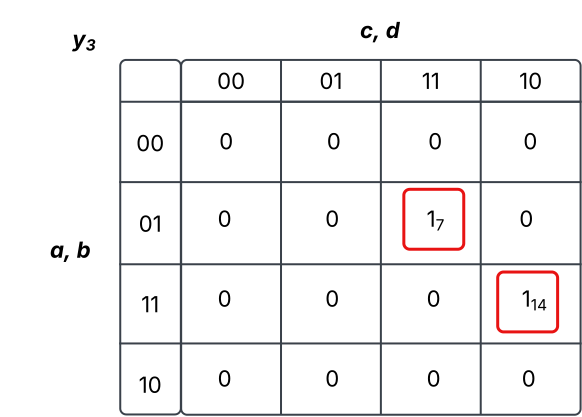
\includegraphics[scale=0.5]{aufgabe 2/img/kv_y3}
    \caption{Karnaugh-Veitch-Diagramm für $y_3$ (Quelle: eigene)}
    \label{fig:kv_y3}
\end{figure}

\begin{figure}
    \centering
    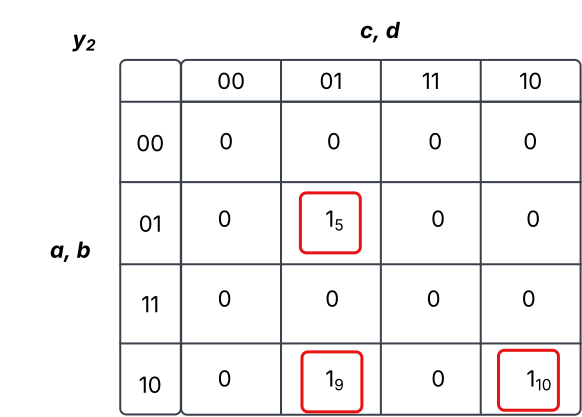
\includegraphics[scale=0.5]{aufgabe 2/img/kv_y2}
    \caption{Karnaugh-Veitch-Diagramm für $y_2$ (Quelle: eigene)}
    \label{fig:kv_y2}
\end{figure}


\begin{figure}
    \centering
    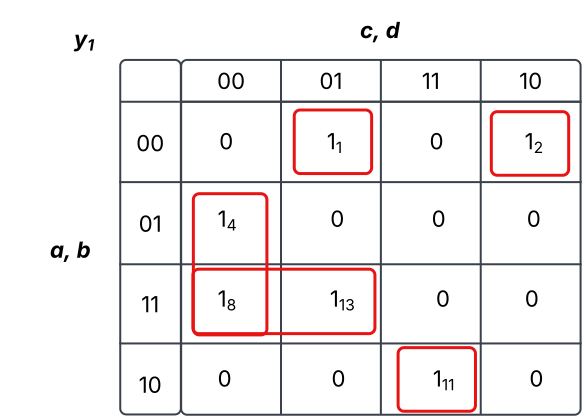
\includegraphics[scale=0.5]{aufgabe 2/img/kv_y1}
    \caption{Karnaugh-Veitch-Diagramm für $y_1$ (Quelle: eigene)}
    \label{fig:kv_y1}
\end{figure}

\noindent
Wie sich aus den Diagrammen ergibt, ist nur eine Minimierung für $y_1$ möglich.
Die Minimierung ist in~\ref{eq:min_y1} angegeben:

\begin{equation}\label{eq:min_y1}
\begin{alignat}{3}
    y_1 =\ &(\neg c \ \land \neg d)\ &&\lor   \\
    &(\phantom{\neg} a \ \land \phantom{\neg} b)\ &&\lor  \\
    &(\neg a \ \land \neg b \ \land \neg c \ \land   \phantom{\neg} d)\ &&\lor  \\
    &(\phantom{\neg} a \ \land \neg b \ \land  \phantom{\neg} c \ \land   \phantom{\neg} d)\ &&\lor  \\
    &(\neg a \ \land \neg b \ \land \phantom{\neg} c \ \land  \neg d)
\end{alignat}
\end{equation}


\section{Teil 3 und Teil 4}

\textit{Geben Sie eine Schaltung für $y_3$ und $y_2$ an.}\\


\noindent
Die Schaltungen für $y_3$ und $y_2$ sind in den Abbildungen~\ref{fig:schaltplan_y3} und~\ref{fig:schaltplan_y2} angegeben.
Hierbei wurden die Gatter - wo angebracht - der Übersicht halber mit mehr als zwei Eingängen angegeben (in Anlehnung an die Darstellung in~\cite[\textbf{Abbildung 24}, 57]{BL22}).

\begin{figure}
    \centering
    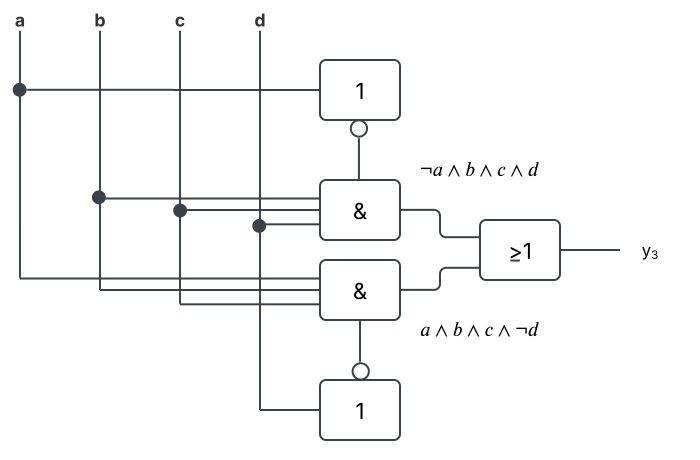
\includegraphics[scale=0.5]{aufgabe 2/img/schaltplan_y3}
    \caption{Schaltung für $y_3$ (Quelle: eigene)}
    \label{fig:schaltplan_y3}
\end{figure}


\begin{figure}
    \centering
    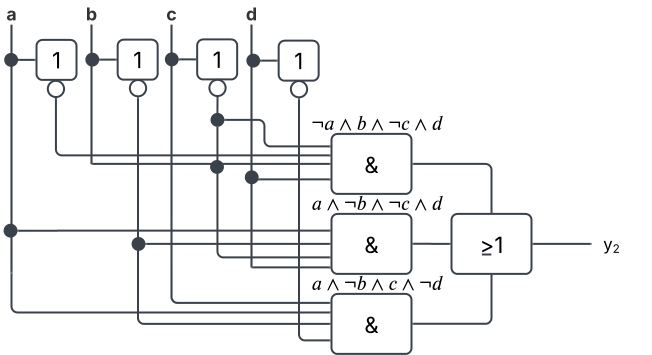
\includegraphics[scale=0.52]{aufgabe 2/img/schaltplan_y2}
    \caption{Schaltung für $y_2$ (Quelle: eigene)}
    \label{fig:schaltplan_y2}
\end{figure}

